\documentclass[../main.tex]{subfiles}

\begin{document}

\chapter{Evaluation}

This chapter evaluates the protocol proposed in chapter~\ref{chap:design}.
Besides the verification of the intended functionality in section~\ref{sec:evaluation-func}, the security and performance of the protocol are investigated in sections \ref{sec:evaluation-sec} and \ref{sec:evaluation-perf}.
This evaluation verifies if the given system requirements (see ~\ref{chap:requirements}) can be fulfilled.

\section{Functionality}
\label{sec:evaluation-func}

This section evaluates the functionality of the designed protocol.
Specifically, the protocol must ensure that the data owner can always access its logs.
It must also allow the data owner to share and revoke access to logs.
Please see section~\ref{functional-requriements} for details.

The protocol requires the following actions:
When the monitor creates a new log it must encrypt it only for the data owner.
Second, whenever the data owner shares or revokes access to a log it must include its own identity into the set of authorized users.
This construction ensures that the data owner is always able to download and decrypt its own logs.

The protocol is based on hybrid encryption.
This means that the log is encrypted with a symmetric encryption scheme.
The used symmetric key is then encrypted for each intended recipient.
Those encrypted keys are attached to the encrypted log.
This allows the construction of logs which can be decrypted by multiple users.
A data owner can re-encrypt the log for specific users because it can always access its logs.
The re-encryption requires the data owner to apply the encryption algorithm.
The provided metadata allow the server to decide if an authorized user is the data owner of a log.
Since the metadata also contains the set of intended receivers, the server can make the shared log available to all recipients. 
This effectively enables the functionality to share and revoke access to the log.

This analysis shows that the designed protocol fulfills all identified functional requirements.
Moreover, the protocol was included into the existing toolchain within the scope of the master thesis.
Section \ref{sec:toolchain-modifications} investigates those changes.
This implementation verifies that the protocol has the intended functionality and can be used in practice.
Moreover, the implemented libraries are heavily tested.
This creates further confidence into their functionality.

\section{Security}
\label{sec:evaluation-sec}

This section investigates the security of the designed protocol.
During requirements engineering three security requirements were identified (details in section ~\ref{security-requriements}).
Each requirement was motivated by an exemplarily attack scenario.
The following sections face the proposed protocol with those attacks.
They reason why the established security mechanisms resist them.

\subsection{Assumptions}

The security of the protocol relies on three fundamental assumptions.
If any of those assumptions is broken the protocol must be considered to be unsecure.

\begin{enumerate}
    \item 
    The protocol has access to a secure PKI.
    Each user requires two key pairs (one for encrypting data and one for signing data).
    It is crucial that each user has exclusive access to its private keys.
    If any other user (or a trusted server) knows a private key of any user the intended E2EE is broken.
    \item 
    The JOSE standard provides secure encryption and signing algorithms.
    Specifically, \verb|A256GCM| and \verb|ECDH-ES+A256KW| must be secure encryption algorithms and \verb|ES256| must be a secure signing algorithm.
    This implies that it is computational infeasible to break those algorithms without knowing the respective keys~\cite{Katz2020}.
    \item 
    The libraries implemented in this thesis rely on language-specific JOSE implementations (details in~\ref{sec:implemented-libraries}).
    It is crucial for the security of the protocol that those libraries follow the definitions of the JOSE protocol.
\end{enumerate}

\subsection{Curious server}
A curious server is a passive attacker which tries to access the logs within the toolchain.
It motivated security requirement S1 which states that only the data owner and explicitly authorized users can access logs.
Recall the attacker Eve who is the database admin of the Overseer server.\todo{cite section}
This section argues why Eve can not access logs if he was not explicitly authorized.

The protocol enforces that only encrypted data is stored in the database.
Both, the monitor creating a log and the data owner sharing a log must encrypt the data before sending it the server.
This ensures that the server only has access to the \emph{JWE} token created by the encryption algorithm.
This \emph{JWE} token is created using hybrid encryption:
First of all, a symmetric key $k$ is randomly generated and the data is encrypted via \verb|A256GCM|.
This is an authenticated symmetric encryption algorithm based on \emph{AES}~\cite[section 4.7]{Jones2015}.
Secondly, this symmetric key is encrypted for each receiver using \verb|ECDH-ES+A256KW|~\cite[section 4.6]{Jones2015}.
This algorithm establishes an ephemeral key between two users which is then used to again encrypt the symmetric key $k$.
The following steps are performed to establish the ephemeral key between a sender and receiver~\cite[100]{Barker2017}:
\begin{enumerate}
    \item 
    The sender must know the static public key of the receiver. 
    In our case this is the public encryption key.
    The receiver must have exclusive access to its static private key.
    In our case this it the private decryption key.
    \item 
    The sender creates a new ephemeral key pair. 
    This key pair must only be once.
    \item 
    The sender sends the public key of the ephemeral key pair to the receiver.
    In our case this data is included within the encrypted key.
    The ephemeral private key must kept secret.
    \item 
    The sender knows the static public key of the receiver and the ephemeral private key of the sender.
    The receiver knows the ephemeral public key of the sender and the static private key of the receiver.
    Thus, the Diffie-Hellman key agreement protocol can be used to compute a shared secret between the sender and the receiver~\cite[section 9.3.6]{Eckert2018}.
    The computation of the shared secret requires either the secret ephemeral key or the secret static key.
    If both are kept secret it is assumed to be computationally infeasible to compute the shared secret~\cite[section 9.3.6]{Eckert2018}.
    \item 
    The shared secret (which is the result of the Diffie-Hellman key agreement protocol) is finally used as input for a key derivation function.
    This function finally computes the ephemeral key between the sender and the receiver.
\end{enumerate}

To access a decrypted log the attacker Eve needs to have access to the symmetric key $k$.
This, however, requires him to have access to any of the ephemeral keys which were used to encrypt $k$.
Eve can compute an ephemeral key only if he has access to either the ephemeral private key of the sender or the static private key of the receiver.
However, those private keys must be kept secret.
If Eve wants to decrypt the log he must either break the encryption algorithms or access a private key.
This, however, contradicts with the assumptions.
If Eve can break an encryption algorithm it is not secure.
If Eve can access a private key of a user the PKI is not secure.
This leads to the conclusion that the malicious database admin Eve can not access decrypted logs.
Only if he was explicitly authorized he can restore the symmetric key $k$ which allows the decryption of a log.


\subsection{Surreptitious forwarding}
Surreptitious forwarding refers to an attack where a malicious user re-encrypts a received log for unintended users (details in section~\ref{sec:surreptitious-forwarding}).
Since such attacks must be detected the security requirement S2 was introduced.
It requires that receivers of encrypted logs can verify that the log was intentionally shared with them.
Recall the attacker described in \todo{cite section}.
Alice shares a log with Eve.
Eve, however, does not stick to the protocol and encrypts the received log for Bob.
Bob must be able to detect this fraud because the log he received was not encrypted by the data owner (Alice).
The following section argues why this attack can be detected.

The mechanism implemented in the protocol to defend this attack is the shared log.
It is a \emph(JWS) token which is signed by the creator of the log.
It is illustrated in figure~\ref{fig:nested-jws}.
It contains the log as a nested \emph{JWS} token.
Moreover, it contains the identity of the creator and the identities of the intended receivers.
Whenever a user successfully decrypted a log it must verify that the shared log is a valid data structure.
\begin{enumerate}
\item 
First of all, the receiver needs to verify if the shared log was signed by the claimed creator.
It fetches the public key of the claimed creator and verifies the cryptographic signature.
If the signature is valid the receiver can be sure that log was signed by the private signing key of the creator.
\item 
The receiver then needs to check if the creator is the data owner. 
This is achieved by checking if the identity of the creator (shared log) is equal to the identity of the data owner in the nested log.
If this holds and if the log was indeed signed by a valid monitor the receiver can be sure that the data-owner crated and signed the shared log.
This, however, does still not pretend surreptitious forwarding.
\item 
In a third step, the receiver must verify if his identity is specified in the list of intended receivers (shared log).
If this is true the receiver knows that the data owner intentionally shared the log with him or her.
This follows from two observations:
First, the receiver can be sure that the shared log was indeed created by the data owner.
Second, the receiver knows that the data owner included his identity into the set of intended receivers.
This gives the receiver confidentiality that no malicious entity re-encrypted the log for him or her.
\end{enumerate}

There is a logical consequence from this validation:
The creator specified in the shared log must have signed the shared log.
The creator specified in the shared log must be equal to the data owner.
Thus, the shared log is only valid if the data owner has shared the signed log.

If Eve wants to forward an encrypted log to the unintended receiver Bob he must either modify the data owner or he must forge a signature of the data owner.
If Eve decides to modify the data owner his attack becomes pointless.
Eve does not want to introduce faked logs.
He wants to forward existing logs to unintended receivers.
Moreover, this requires Eve to be a valid monitor because only they are allowed to sign logs.
On the other hand, Eve might try to forge a signature of the data owner.
However, this contradicts with the assumptions.
To successfully forge a signature Bob either has access to the private signing key of the data owner or he breaks the signing algorithm.
The first breaks the security of the assumed PKI.
The second breaks the security of the chosen signing algorithm.
There is no way for Eve to forward a received log to unintended recipients if those recipients validate the shared log correctly.


Again consider Eve who wants to forward encrypted logs to the unintended receiver Bob.
Eve has access to the log which was singed by a monitor.
He can not sign this log by himself because he is not a valid monitor.
Moreover, Eve does not want to introduce faked logs.
He wants to forward existing logs to unintended receivers.
Thus, his attack relies on the log which was signed by a valid monitor.
To succeed he must create a shared log which passes the validation of Bob.
Specifically, Bob's identity must included in the list of intended receivers.
Assume Eve creates a shared log which contains the existing log.
Eve can specify itself as creator and sign the log with his private signing key.
Bob will detect this fraud because the identity of the creator (Eve) is not equal to the identity of the data owner (Alice).
Hence, Bob must specify Alice as creator of the shared log.
Bob will also detect this fraud because in this case Eve signs the shared log which claims to be created by Alice.
Eve can only share the log with Bob if he knows the private signing key of Alice.
This allows him to specify the creator to be the Alice and to successfully sign the shared log.
However, this contradicts with the assumption of a valid PKI where each user has exclusive access to its keys.


\subsection{Malicious data owner}

\section{Performance}
\label{sec:evaluation-perf}

\subsection{Methodology}
\subsection{Results}

\begin{figure}[ht]
    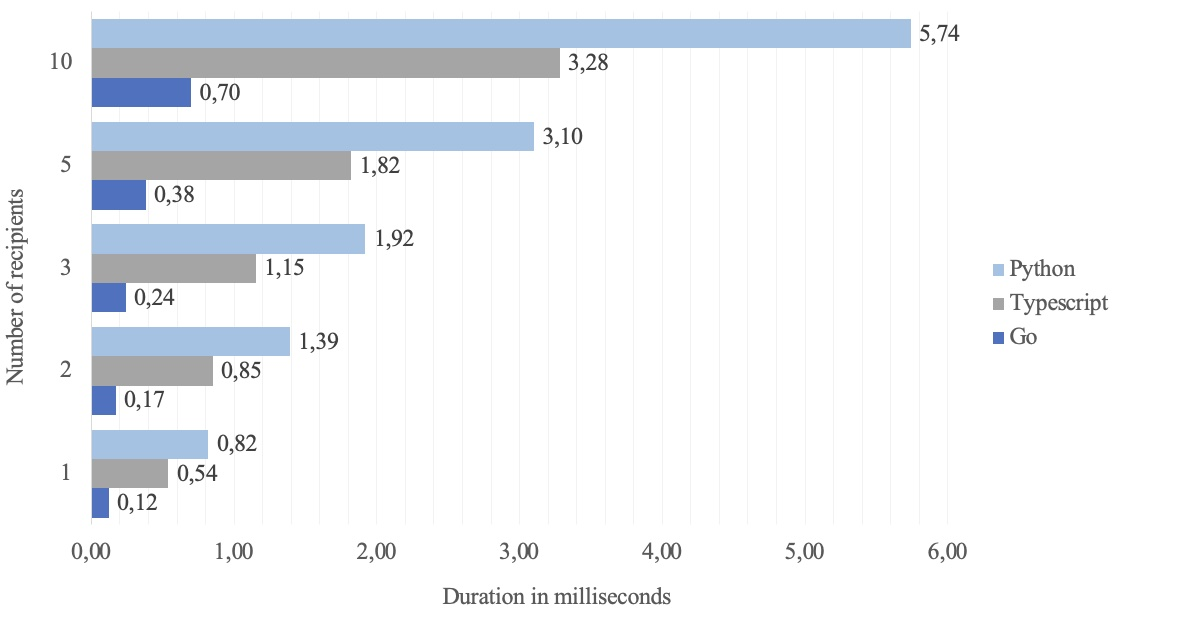
\includegraphics[scale=0.3]{../img/07/performance_tests.jpg}
    \centering
    \caption{This figure visualizes the duration of encrypting the same log for a different number of recipients.}
    \label{fig:mutual_encryption}
\end{figure}

\end{document}